\documentclass{article} % For LaTeX2e
\usepackage{nips15submit_e,times}
\usepackage{hyperref}
\usepackage{url}
\usepackage{amsmath}
\usepackage{amssymb}
\usepackage{graphicx} 
%\documentstyle[nips14submit_09,times,art10]{article} % For LaTeX 2.09

\usepackage{algpseudocode}

\title{Image Processing Using Convolution Matrices - Multithreaded CPU vs FPGA}


\author{
Preston Scott\\
% \thanks{ Use footnote for providing further information
% about author (webpage, alternative address)---\emph{not} for acknowledging
% funding agencies.} \\
Department of Computer Science\\
NC State University\\
Raleigh, NC 27695 \\
\texttt{pdscott2@ncsu.edu} \\
% \And
% Coauthor \\
% Affiliation \\
% Address \\
% \texttt{email} \\
% \AND
% Coauthor \\
% Affiliation \\
% Address \\
% \texttt{email} \\
% \And
% Coauthor \\
% Affiliation \\
% Address \\
% \texttt{email} \\
% \And
% Coauthor \\
% Affiliation \\
% Address \\
% \texttt{email} \\
% (if needed)\\
}

% The \author macro works with any number of authors. There are two commands
% used to separate the names and addresses of multiple authors: \And and \AND.
%
% Using \And between authors leaves it to \LaTeX{} to determine where to break
% the lines. Using \AND forces a linebreak at that point. So, if \LaTeX{}
% puts 3 of 4 authors names on the first line, and the last on the second
% line, try using \AND instead of \And before the third author name.

\newcommand{\fix}{\marginpar{FIX}}
\newcommand{\new}{\marginpar{NEW}}

\nipsfinalcopy % Uncomment for camera-ready version

\begin{document}


\maketitle

\begin{abstract}
With the prevalence of smart phone cameras and other mobile camera devices, image processing has become an important focus area for research.  Without the benefit of large, expensive optics and controls, mobile cameras must increasingly solve problems computationally. Modern mobile cameras use image processing algorithms for every step of the imaging process - helping users to automatically focus on objects during image capture and also enhance images via post processing after they are stored. Third party applications such as Instagram have gained enormous popularity from their ability to quickly turn ordinary photographs into works of art through creative use of image filtering. Since image processing has become so ubiquitous, it is important that the supporting algorithms as as efficient as possible.  In this paper, we will discuss one of the more basic forms of image processing - the application of a convolution matrix or kernel to an image. In particular, we shall explore the possibilities of speeding up the convolution process by 1) using multiple threads on different CPU cores and 2) exploiting even more parallelism using an FPGA.[1]   

\end{abstract}

\section{Motivation / Background}
Recent statistics reveal that 77\% of Americans now own a smart phone. [2] This means that there are more than 200 million people walking around with cameras in their pockets. These cameras are equipped with incredibly advanced multi-core processors, beautiful high-resolution screens, and lightning fast access to the Internet.  One thing that they are not equipped with, however, is a large optical lens.  Necessarily, mobile cameras must be small and easy to fit into compact enclosure. The small diameter of the mobile camera lens means that it cannot collect as much light as a traditional camera lens. With so few photons to work with, it becomes very challenging to produce noise-free images.  Mobile cameras must also fit into the increasingly thin smart phone body.  This thinness places a limit on the focal length of the lens which impacts the amount of magnification the lens can provide.  \\
\\
With all of these limitations on the design of the mobile camera, it is surprising that decent images can be captured at all.  Yet mobile photographers are producing some of the most beautiful imagery ever captured.  How are these tiny devices capable of producing imagery comparable to large specialty cameras? The answer lies in how the images are processed.  Without the benefit of physics and optics, mobile cameras must find different solutions to problems by doing what they do best - computations.  Between the time a user snaps an image and the time it shows up on the screen milliseconds later, the internal CPU of the mobile camera has already read and written every pixel within the image several times - optimizing for brightness, color, and clarity. \\
\\
The main drawbacks of relying on computational solutions are time and energy.  With every pass over the pixels, the CPU consumes precious time and depletes battery life. These problems may lead to a bad user experience or, even worse, may result in a missed photo opportunity. Every CPU cycle spent working on the last photo taken means that it is not available for the next photo.  It is for this reason that image processing algorithms have become increasingly important. If our devices must rely on intensive computations to do their work, then we must ensure that we optimize our algorithms such that every computation is as efficient as possible.  \\
\\
\begin{figure}[ht!]
\centering
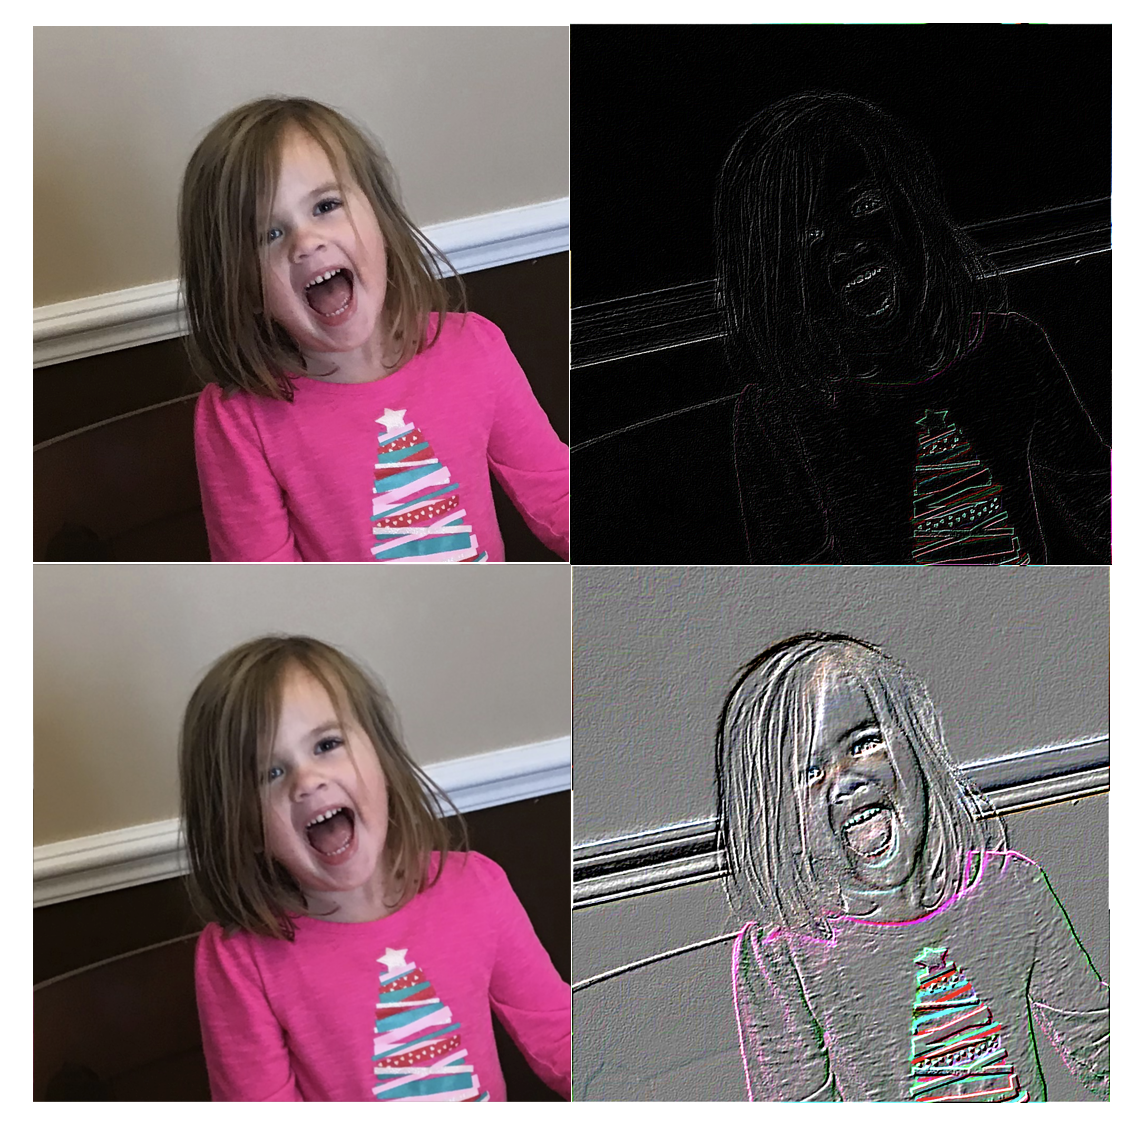
\includegraphics[width=120mm]{filters.png}
\caption{Imaging effects possible using different convolutional matrices. Clockwise from top left - original, edge filter, Gaussian blur, embossing. \label{overflow}}
\end{figure}
\\
One of the primary tools used in processing images is that convolution matrix (sometimes referred to as kernel). [3] Using this approach, one examines every pixel within the image and rewrites its values based on an average of the neighboring pixels.  As shown in Figure 1, this approach is remarkably versatile and can be tuned to a) highlight edges within an image 2) perform blurring of various degrees or 3) produce creative effects such as embossing.  Figure 2 below shows the concept behind a convolution matrix.  The bitmap image on the left represents a large array of pixels within an image. Each pixel has separate values for its red, green, and blue components. The pixel of interest for this snapshot in time is the middle pixel (5) with values R5, G5, and B5 for its red, green, and blue components.  To calculate the new value of pixel 5, it is averaged with the values of its neighboring pixels. \\
\\
The exact weighting of this averaging is given by the convolution matrix on the right. The elements of the matrix represent the multiplicative factors to be applied to each corresponding pixel in the image. In this Gaussian blur example, the center pixel is weighted more heavily with a multiplicative factor of 4. As one gets further away from the middle pixel, the weightings decrease according to a Gaussian distribution.  The complete calculation is shown for the new red component of pixel 5.  As shown, the new red component of a given pixel is a combination of the red components of all neighboring pixels and itself. Similar computations must be done for the green and blue components.  At the end, the final sum multiplied a normalization factor (in this case 1/16). \\

\begin{figure}[ht!]
\centering
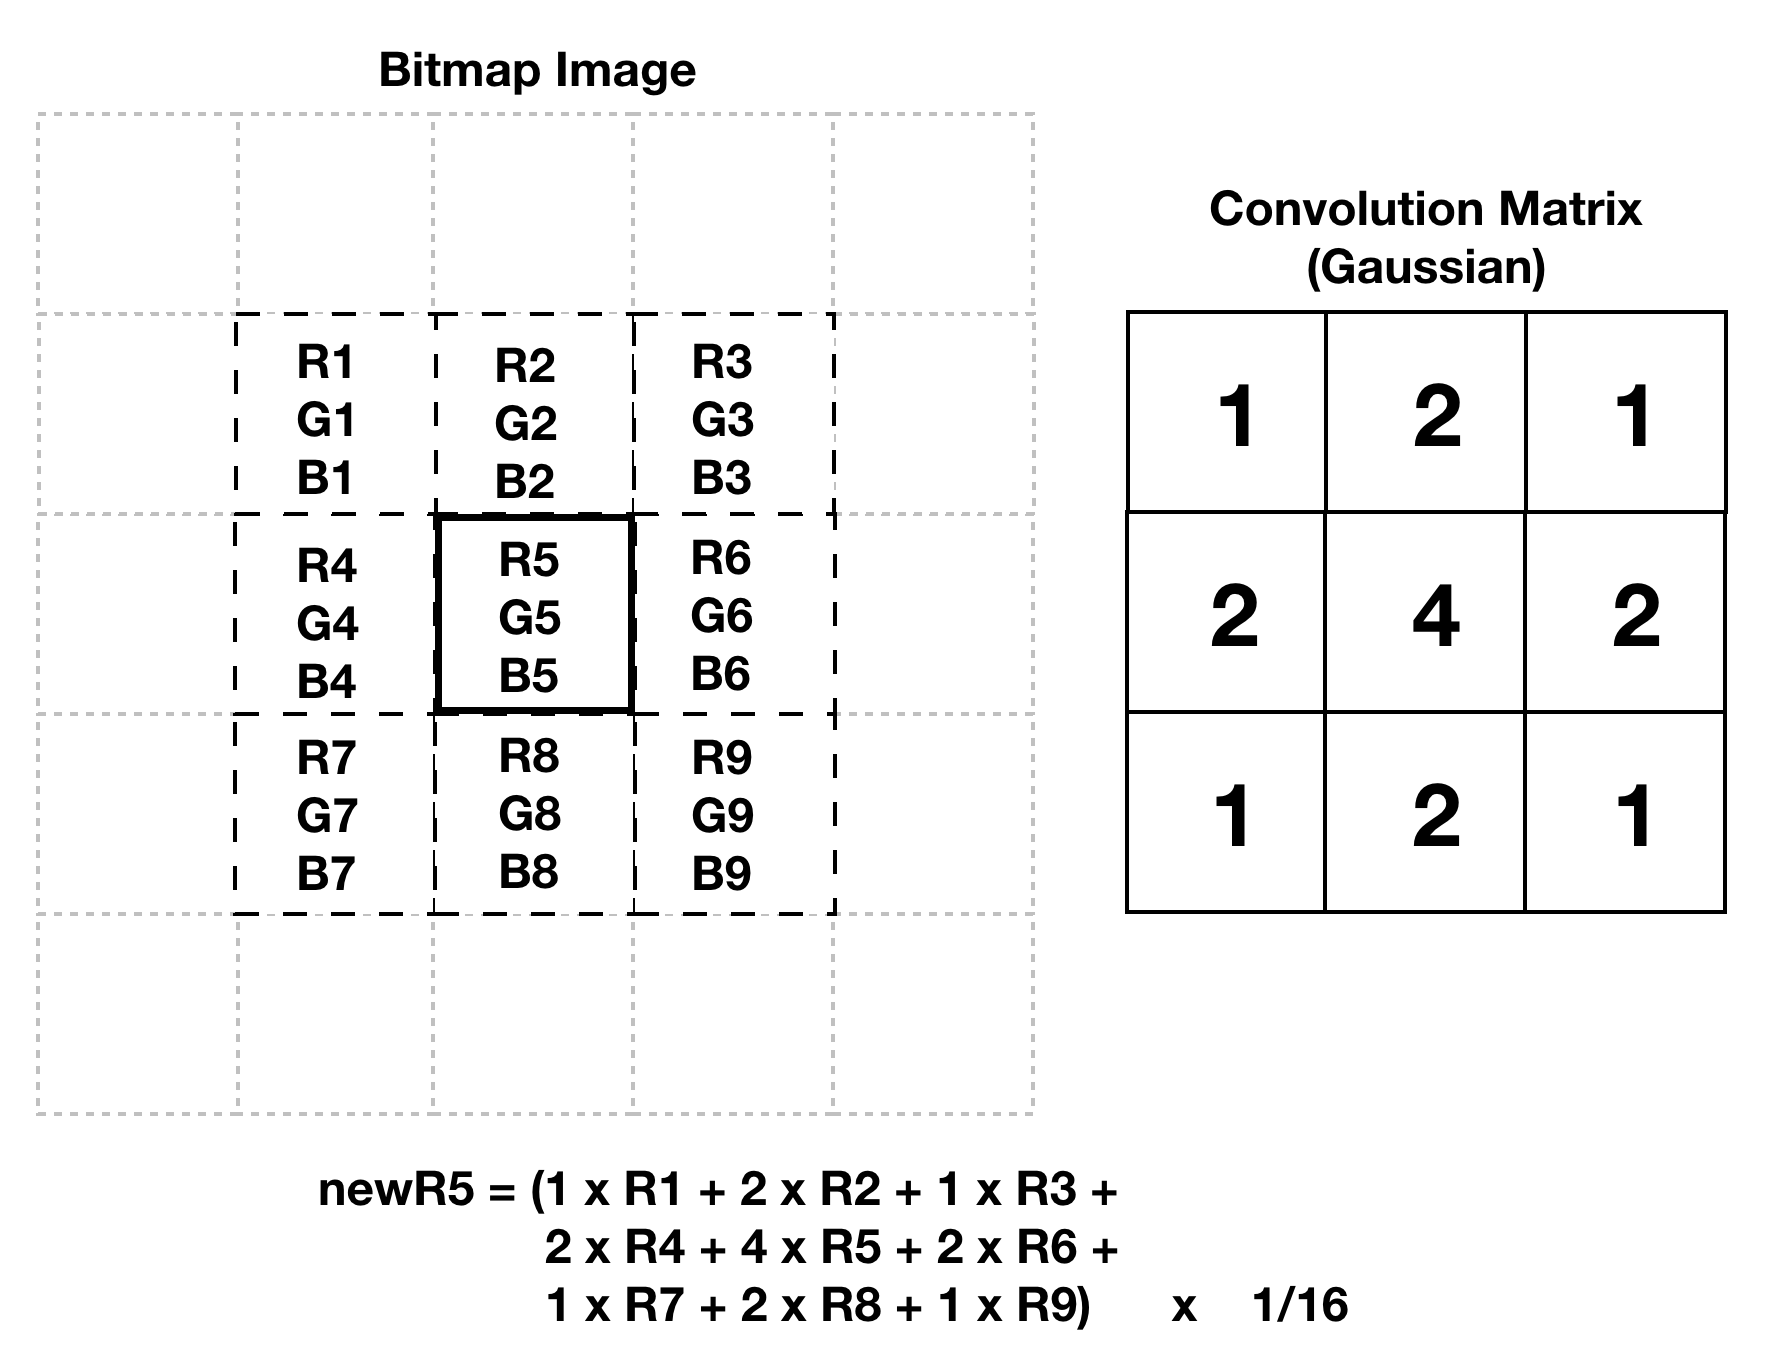
\includegraphics[width=120mm]{matrix.png}
\caption{Conceptual diagram of the convolutional filtering approach showing raw image pixels (left) and convolution matrix (right).\label{overflow}}
\end{figure}

\section{Methods / Architectural Solutions}
The convolutional filter, in its simplest approach, is an iterative problem which can be defined algorithmically as follows: \\
 \begin{algorithmic}
 \Function{Filter}{in, out, w, h, n}
 	\For {Each column 0 to w-1}
		\For {Each row 0 to h-1}
	    	\For {Each filterColumn 0 to n-1}
	    		\For {Each filterRow 0 to n-1}
					\State {pixelX = (column - n / 2 + filterColumn + w) mod w}
					\State {pixelY = (row - n / 2 + filterRow + h) mod w}
					\State {red += in[pixelY][pixelX].red * filter[filterRow][filterColumn]}
					\State {blue += in[pixelY][pixelX].green * filter[filterRow][filterColumn]}
					\State {green += in[pixelY][pixelX].blue * filter[filterRow][filterColumn]}
				\EndFor
			\EndFor
		\State {out[row * w + col].red = red}
		\State {out[row * w + col].green = green}
		\State {out[row * w + col].blue = blue}
		\EndFor
	\EndFor
\EndFunction
\end{algorithmic}

The filter function is called with parameter in, out, w, h, and n, which represent the source image, destination image, image width, image height, and filter size, respectively. The quadruple nested loops combine to make this algorithm $O(w*h*n^2)$. An important aspect of this algorithm, however, is that all of the computations are independent of each other. That is, none of the computations for a given pixel rely on the computations for any other pixel.  In that sense, the pixels can be traversed in any order as long as each is processed eventually. \\
\\
An important consequence of this pixel independence is that this algorithm can be parallelized. Each core of a multi-core CPU may receive disjoint pieces of the same image to be processed in parallel and then stitched back together at the end.  More extreme parallelism can be achieved by passing each separate pixel computation to a separate work item on an FPGA. 

\section{Design}
Three sets of experiments were conducted to assess different methods of parallelization for image processing.  In the first experiment, an eight core x86 CPU was used to quantify the speedup achievable using multiple threads. The size of the convolution matrix was also considered as a variable in this experiment.  In the second experiment, a dual core ARM CPU was used to quantify multi-threaded speedup.  In the final experiment, an FPGA was used to assess speedup achievable using FPGA work units. The experimental plan is given in Table 1. 

\begin{table}[h!]
\centering
\begin{tabular}{|c|l|l|}
\hline
\textbf{Experiment} & \textbf{Architectural Details} & \textbf{Purpose} \\
\hline\hline
1 & 2.6GHz Intel 8 Core i7  & Evaluate multi-thread speedup on x86 \\
2 & 925MHz ARM Cortex-A9 Dual Core & Evaluate multi-thread speedup on ARM  \\
3 & Cyclone V FPGA & Evaluate speedup using FPGA \\
\hline
\end{tabular}
\caption{Experimental Plan}
\end{table}

% \begin{table}[h!]
% \centering
% \begin{tabular}{|c|c|l|}
% \hline
% \textbf{Experiment} & \textbf{Architectural Details} & \textbf{Variables}  \\
% \hline\hline
% 1 & 2.6GHz Intel 8 Core i7 & number of threads, matrix size \\
% 2 & Evaluate multi-thread speedup on ARM  & number of threads \\
% 3 & Evaluate speedup using FPGA & -  \\
% \hline
% \end{tabular}
% \caption{Experimental Plan}
% \end{table}

\section{Methodology}
\subsection{General Procedure}
Although there are many different types of image file formats, they all have certain commonalities. All file formats contain a header with meta-data followed by a long array of pixel information. For each pixel, files must specify values for the red, green, and blue components of that pixel. Optionally, the pixel may have an alpha component, which specifies the transparency of the pixel.  Pixel information may be stored as 1, 4, 8, 16, 24, or 32 bit entities. Most modern image formats house pixel information as 32 bit integers with each red, green, blue, and alpha component occupying one byte. \\
\\
For the purposes of this project, we will use the BMP file format.  This format has the advantage of being easy to read since there is no compression involved.  The standard BMP file has a 54 byte header followed by an array of 32 but pixel values.  Pertinent header fields are listed in Table 2 [4].

\begin{table}[h!]
\centering
\begin{tabular}{|c|c|l|}
\hline
\textbf{Decimal Offset} & \textbf{Size (bytes)} & \textbf{Purpose} \\
\hline\hline
0 & 2 & BMP variant \\
2 & 4  & Size of image in bytes \\
10 & 4 & The offset where pixel data begins  \\
18 & 4 & The image width in pixels  \\
22 & 4 & The image height in pixels  \\
28 & 4 & The number of bits per pixel  \\
\hline
\end{tabular}
\caption{Bitmap header fields}
\end{table}

\subsection{Multi-Threading}
The data portion of an image file is simply a list of 32 bit numbers that give the color information for each pixel.  Pixels are listed by rastering from left to right and from top to bottom.  A naive implementation of multi-threading would simply cut an n-pixel image in half, sending n/2 pixels to each CPU core.  This approach yields a slightly disappointing result based on how the algorithm handles edges. \\
\\
Every convolution algorithm must have an approach for dealing with edge pixels which have no neighbors. The approach used in the pseudo-code above is to use a "wrap-around" technique, as indicated by the modular arithmetic in the pixel coordinate calculations.  Using this approach, an edge pixel with no neighbors on one side simply pulls in a neighbor from the other side of the image.  This approach works well, but causes problems when processing pieces of an image in parallel. As shown in Figure 3, the two separately processed data streams are pieced together, they form a boundary artifact at their adjacent edges.   

\begin{figure}[ht!]
\centering
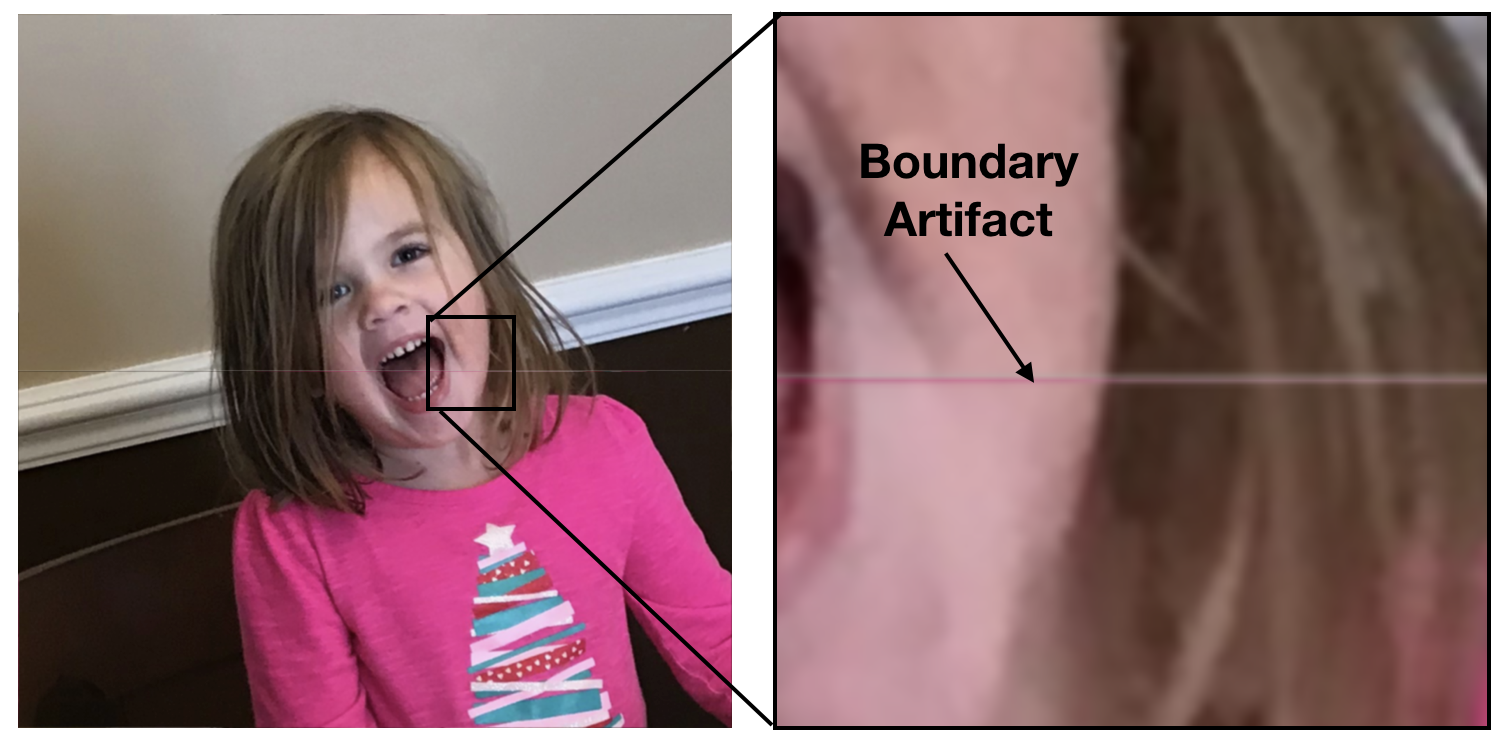
\includegraphics[width=120mm]{boundary.png}
\caption{Processing artifact caused by piecing together two separately processed halves of an image.\label{overflow}}
\end{figure}


To avoid this problem, one must be careful in 1) selecting which data to send to the filtering algorithm for each piece of the image and in 2) how each set of data is parsed within the filtering algorithm.  Figure 4 shows the proper way to separate an image into pieces for parallel algorithm.  For each image fragment, buffer rows along the axis of intersection should be including in dataset sent to the filtering algorithm.  The number of required buffer rows depends on the size of the convolution matrix (e.g. a 5 x 5 matrix requires a two row buffer on each edge). \\

\begin{figure}[ht!]
\centering
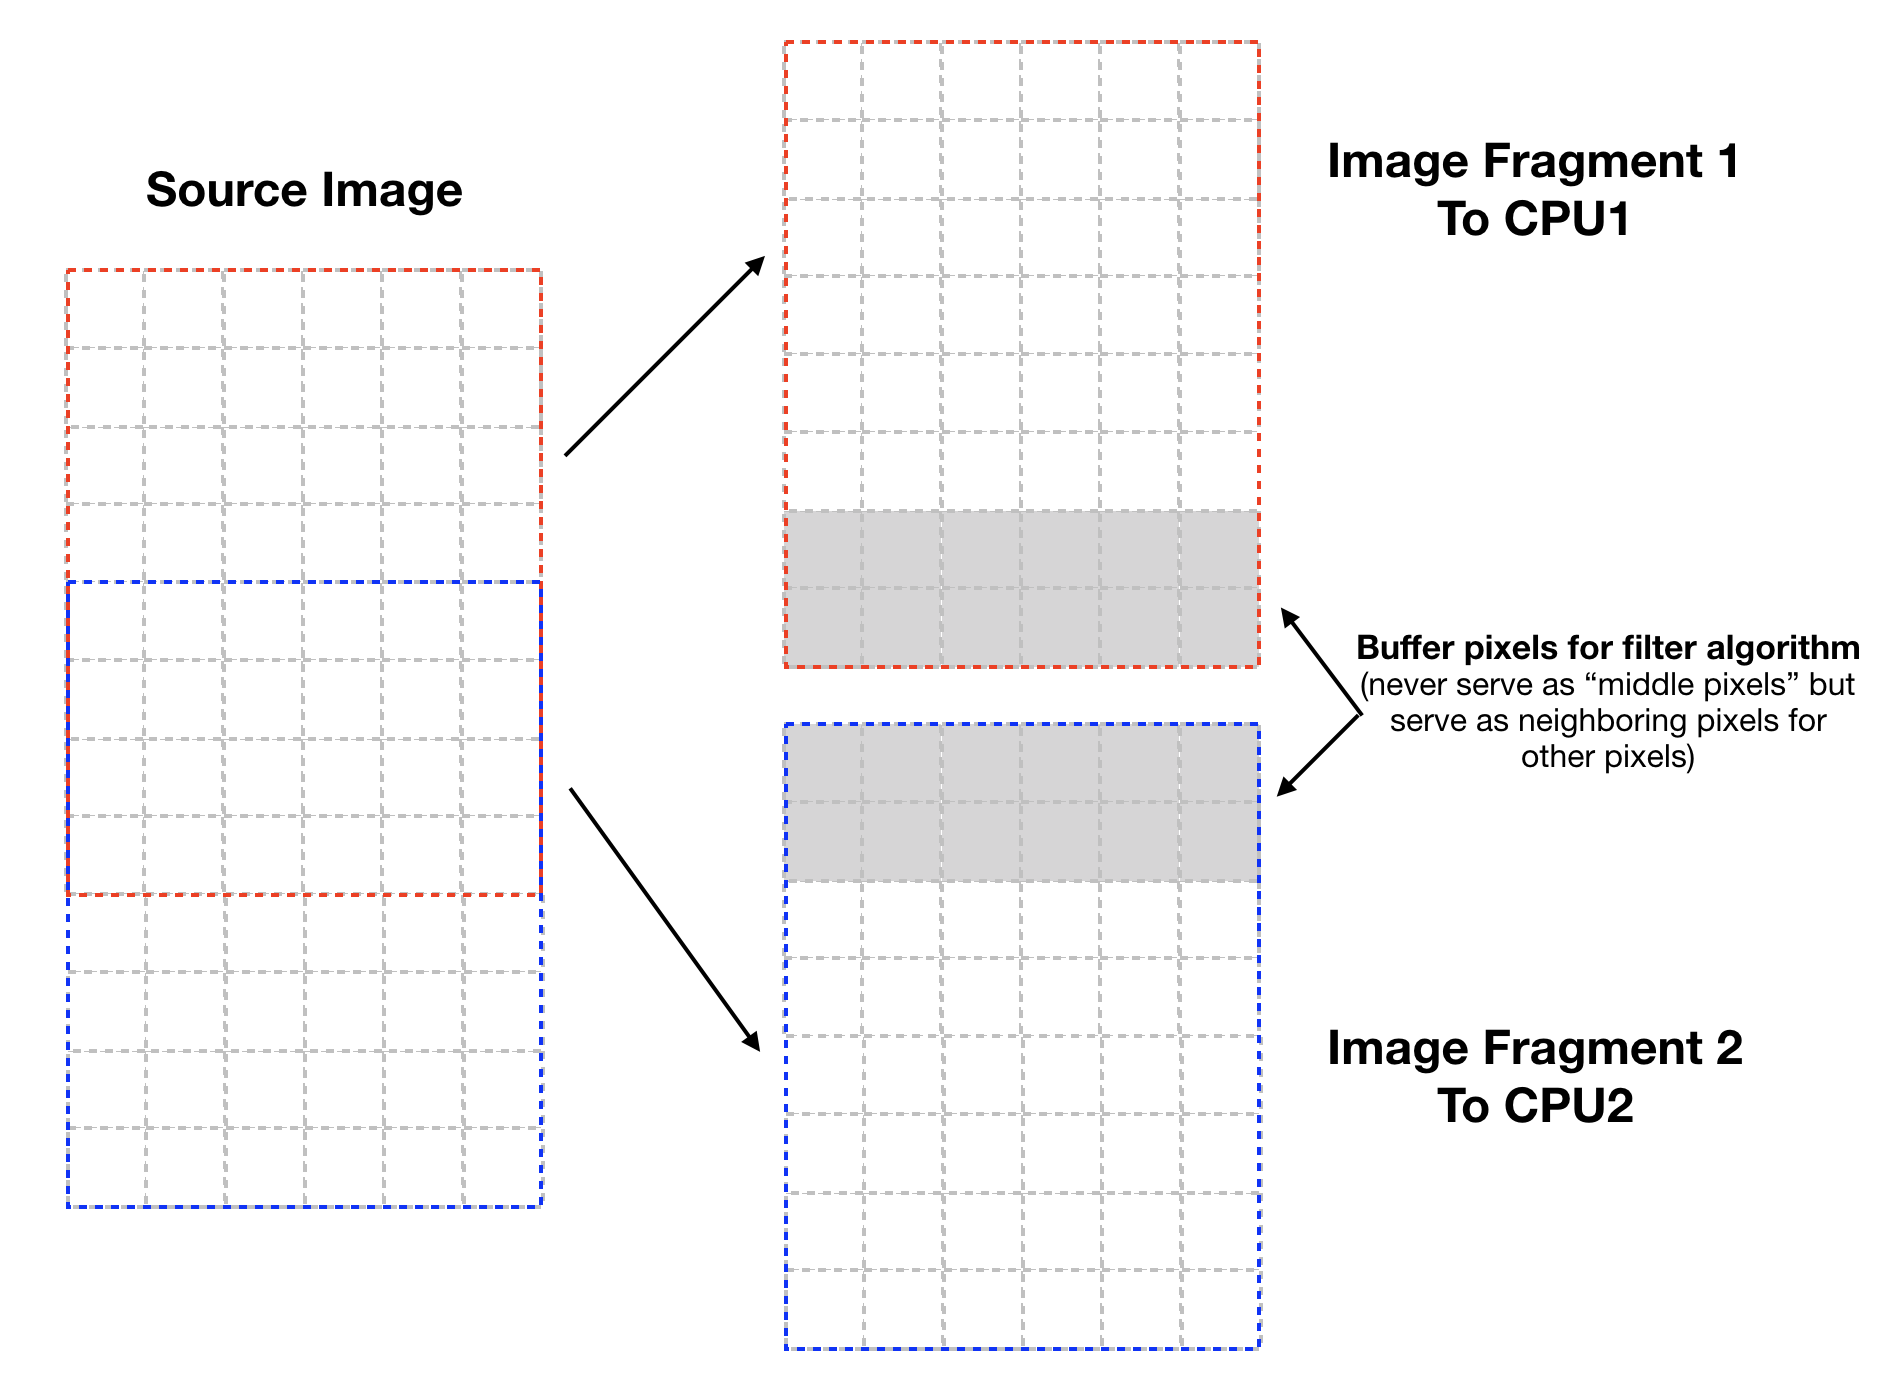
\includegraphics[width=120mm]{buffer.png}
\caption{Diagram showing proper splicing of image fragments for multi-threaded processing.\label{overflow}}
\end{figure}

Once the data is selected, the filtering algorithm must then be slightly modified to ignore the buffer rows in selecting pixels of interest.  The buffer row pixels are never selected to serve as the "middle" pixel during the iteration, but are present to serve as neighbor pixels for the actual pixels of interest.

\subsection{FPGA Programming}
The modifications necessary for FPGA processing were straight-forward. The FPGA was configured such that each work unit would handle the computations for a given x-y location within the image.  By defining the problem in this way, the two outer loops within the filtering algorithm could be eliminated.  The entire source and destination pixel arrays were written to the FPGA so there was no problem with edge effects.  One all portions of the processing were finished by the FPGA, the destination image data was rewritten back to the host.  

\section{Results}
\subsection{x86 Multi-Threading}
The first round of testing was conducted on an x86 based processor using increasing numbers of threads. The baseline performance was defined to be the single threaded performance and the amount of speedup was documented as the number of threads was increased.

\begin{table}[h!]
\centering
\begin{tabular}{|c|c|c|}
\hline
\textbf{Number of Threads} & \textbf{Execution Time (ms)} & \textbf{Speedup} \\
\hline\hline
1 & 8,451 & - \\
2 & 4,413 & 1.91  \\
3 & 2.964 & 2.85  \\
4 & 2,376 & 3.55  \\
5 & 2,356 & 3.58  \\
6 & 2,126 & 3.97  \\
7 & 2,026 & 4.17  \\
8 & 1,934 & 4.36  \\
\hline
\end{tabular}
\caption{Execution time vs number of threads for x86}
\end{table}



\begin{table}[h!]
\centering
\begin{tabular}{|c|c|c|c|}
\hline
\textbf{Number of Threads} & \textbf{Matrix Size} & \textbf{Execution Time (ms)} & \textbf{Speedup} \\
\hline\hline
1 & 3 x 3 & 4,074 & 2.08 \\
1 & 5 x 5 & 8,485 & -  \\  
1 & 7 x 7 & 14,492 & 0.59 \\ 
1 & 9 x 9 & 22,509 &  0.38 \\ 
1 & 11 x 11 & 35,898 &  0.24\\ 
\hline
\end{tabular}
\caption{Execution time vs matrix size for x86}
\end{table}

Table 3 shows the results of the multi-threading experiment.  For this testing, a standard 5 x 5 convolution matrix was used. As shown, the speedup improved dramatically with the addition of additional threads.  After the third thread, however, performance began to asymptote and a point of diminishing returns was reached.  This is presumably because of a) the increasing overhead of launching and maintaining threads and b) the increasing inability to find an idle processor core free enough to devote entirely to the task of image processing.  \\
\\
Table 4 shows the results of matrix size vs execution time. The impact of matrix size on execution time was predictable.  The execution time increase  was roughly proportional to the number of computations yielded by the matrix size. Since this influence of matrix size proved to be predictable, a standard 5 x 5 matrix was used for the remainder of the experiments.\\

\subsection{ARM Multi-Threading}
Table 5 shows the results of the image processing experimentation on the ARM dual core processor.  The execution time of the single threaded routine increased substantially from the x86 execution time.  This increase was roughly proportional to difference in CPU cycle time between the processors.  However, since the instruction sets were also different between the two processors, this undoubtedly also played a role. There was little difference in performance based on the type of convolution matrix used (e.g. the actual values within the matrix). 
\begin{table}[h!]
\centering
\begin{tabular}{|c|c|c|c|}
\hline
\textbf{Number of Threads} & \textbf{Filter} & \textbf{Execution Time (ms)} & \textbf{Speedup} \\
\hline\hline
1 & Identity & 21,948 & - \\
2 & Identity & 11,413 & 1.92  \\
1 & Edge Detection & 22,205 & - \\
2 & Edge Detection & 11,537 & 1.90 \\
1 & Gaussian Blur & 21,860 & - \\
2 & Gaussian Blur & 11,393 & 1.92 \\
1 & Emboss & 21,629 & - \\
2 & Emboss & 11,425 & 1.92 \\
\hline
\end{tabular}
\caption{Execution time vs matrix size for x86}
\end{table}

\subsection{FPGA Computation}
The results of the FPGA computations are shown in Table 6.  There was a considerable speedup achieved from the ARM single thread baseline.  The performance was undoubtedly capped by the overhead of reading and writing the data to the FPGA board.

\begin{table}[h!]
\centering
\begin{tabular}{|c|c|c|}
\hline
\textbf{Filter} & \textbf{Execution Time (ms)} & \textbf{Speedup vs ARM Single Core} \\
\hline\hline
Identity & 3273 & 6.70 \\
Edge Detection & 3307 & 6.71 \\
Gaussian Blur & 3236 & 6.75 \\
Emboss & 3159 & 6,84 \\
\hline
\end{tabular}
\caption{Execution time vs matrix size for x86}
\end{table}
\section{Conclusions}
This project showed the increase in performance which can be achieved in image processing by exploiting different forms of parallelism in the execution of the computations.  Performance increases on a standard desktop CPU can be easily achieved by processing different parts of the image on different cores. Depending on the CPU, a performance asymptote is reached after the number of threads exceeds the number of available CPUs. The size of the convolution matrix was also shown to be a significant factor in the execution time, albeit one that the user may not be able to control. Care should be taken to ensure that the convolution matrix is as small as possible.  The actual values within the convolution matrix were not significant factors in the execution time.  \\
\\
Substantial speedups were also noted on the ARM CPU by using multiple threads to process images. Since most mobile cameras use ARM processors, the ARM performance may be the most realistic environment for experimentation. Speedups of 2x were achieved by using both of the CPU cores instead of one.  \\
\\
FPGA performance was also surprisingly good - showing a 6x speedup vs the single core ARM solution. FPGA solutions may not be realistic on mobile phones, but the performance does address the possibility of what might be achieved on specialized ASIC or GPU.

\section*{References}
\small{
[1] Code for this project https://github.com/pdscott/ImageFilter . 

[2] http://www.pewinternet.org/fact-sheet/mobile/ .

[3] Russ, John C., The Image Processing Handbook, Seventh Edition. CRC Press.

[4] https://en.wikipedia.org/wiki/BMP\_file\_format . 

}

\end{document}